\section{Homonuclear Diatomic Molecules}

The focus regarding homonuclear diatomic molecules, from here on referred to as molecules, has been similar to the focus on atoms, with the exception of parameterizing atomic forces which can be applied in molecular dynamics simulations. The implementation of molecular systems were achieved by adding ~200 lines of code. This fact by it self represents a successful result regarding the code structure. For details regarding the transformation from atomic - to molecular systems, see Section \ref{sec:homoMolecules}.

\subsection{Ground State Energies}
 
\begin{table}
\begin{center}
\begin{tabular}{lrccrlrrc}
Molecule & $R$ & & \qquad & $E_\mathrm{VMC}$ & & \qquad $E_\mathrm{DMC}$ & \qquad\,\, Expt. & \qquad $\epsilon_\mathrm{rel}$\\
\hline\hline
\ \\
$\mathrm{H_2}$ & 1.4   & &\qquad & -1.1551(3)    & \qquad   & -1.1745(3)   & \qquad $-1.1746$      & \qquad $8.51\cdot 10^{-5}$ \\
\ \\
$\mathrm{Li_2}$& 5.051 & &\qquad & -14.743(3)    & \qquad   & -14.988(2)   & \qquad $-14.99544$    & \qquad $4.96\cdot 10^{-4}$ \\
\ \\
$\mathrm{Be_2}$& 4.63  & &\qquad & -28.666(5)    & \qquad   & -29.301(5)   & \qquad $-29.33854(5)$ & \qquad $1.28\cdot 10^{-3}$  \\
\ \\
$\mathrm{B_2}$ & 3.005 & &\qquad & -47.746(7)    & \qquad   & -49.155(5)   & \qquad $-49.4184$     & \qquad $5.33\cdot 10^{-3}$  \\
\ \\
$\mathrm{C_2}$ & 2.3481& &\qquad & -72.590(8)    & \qquad   & -74.95(1)    & \qquad $-75.923(5)$   & \qquad $1.28\cdot 10^{-2}$  \\
\ \\
$\mathrm{N_2}$ & 2.068 & &\qquad & -102.78(1)    & \qquad   & -106.05(2)   & \qquad $-109.5423$    & \qquad $3.19\cdot 10^{-2}$  \\
\ \\
$\mathrm{O_2}$ & 2.282 & &\qquad & -143.97(2)    & \qquad   & -148.53(2)   & \qquad $-150.3268$    & \qquad $1.2\cdot 10^{-2}$  \\
\ \\
\end{tabular}
\caption{Ground state energies for homonuclear diatomic molecules calculated using VMC and DMC. The distance between the atoms $R$ are taken from Ref. \cite{H_He_exact} for $\mathrm{H_2}$ and from Ref. \cite{UmrigarMolecules} for $\mathrm{Li_2}$ to $\mathrm{O_2}$. The experimental energies are taken from Ref. \cite{H_He_exact} for $\mathrm{H_2}$ and from Ref. \cite{ExactMolecules} for $\mathrm{Li_2}$ to $\mathrm{O_2}$. As expected DMC is closer to the experimental energy than VMC. $\epsilon_\mathrm{rel} = |E_\mathrm{DMC} - \mathrm{Expt.}|/|\mathrm{Expt.}|$ denotes the relative error between the DMC result and the experimental value. As expected, this error increase with the atomic number.}
\label{tab:MoleculesRes}
\end{center}
\end{table}

Table \ref{tab:MoleculesRes} lists the VMC and DMC results with the corresponding experimental energies for $\mathrm{H_2}$ through $\mathrm{O_2}$. As expected, the two particle result is very close to the experimental value with the same precision as the result for the Helium atom in Table \ref{tab:AtomsRes}. The relative error from the experimental energy increase with the atomic number, and is far higher than the errors in the case of pure atoms. This is a result of the trial wave function being worse due to the fact that it does not account for the nucleus-nucleus interaction term in the molecular Hamiltonian. Nevertheless, taking the simple nature of the trial wave function into consideration, the calculated energies are satisfyingly close to the experimental ones. 

As with atoms, these energies were calculated on a single node, resulting in a rather big statistical error in DMC. Doing the calculations on a supercomputer with an increase in the number of walkers could decrease this error.

\subsection{One-body densities}

Figure \ref{fig:OBD_Molecules} presents the one-body densities of $\mathrm{Li_2}$, $\mathrm{Be_2}$ and $\mathrm{O_2}$. The densities have strong peaks located at a distance equal to half of the listed core separation $R$, indicating that the nucleus interaction still dominates the general shape of the distributions. From the figure it is clear that most of the electrons are on the side facing the opposite core, leading to the conclusion that the molecules share a covalent bond \cite{UniversityPhysics}. This is especially clear in the case of the oxygen molecule, where there is a small formation of electrons on the inner side of the nuclei.

\vspace{2cm}
\renewcommand\floatpagefraction{.9}
\begin{figure}[h]
 \begin{center}
   \subfigure{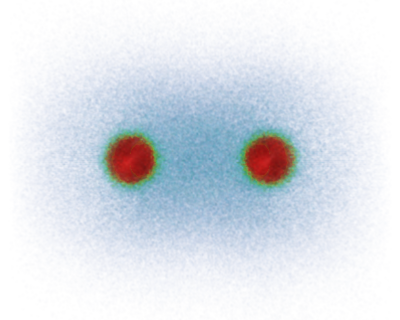
\includegraphics[scale=0.4]{../Graphics/OBD/OBD_MOL/Li2_3D.png}} 
   \subfigure{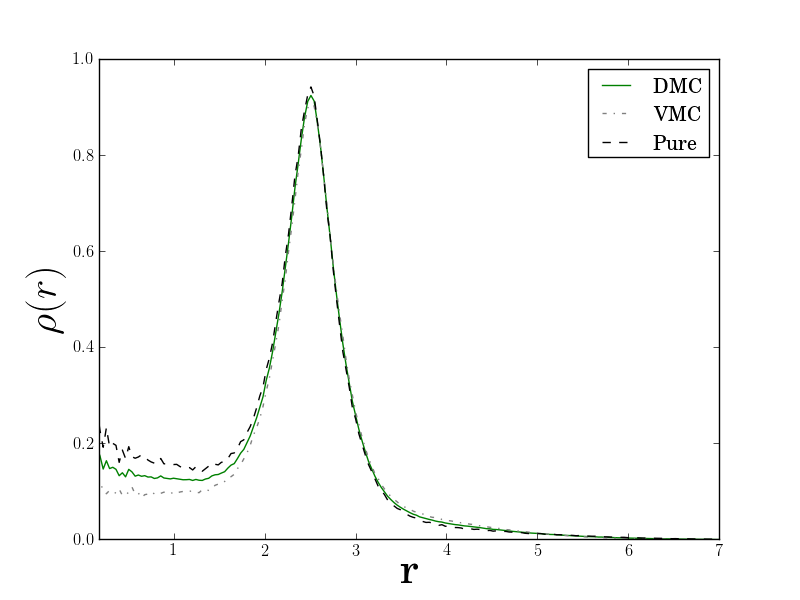
\includegraphics[scale=0.3]{../Graphics/OBD/OBD_MOL/Li2_2D.png}}  \\
   \subfigure{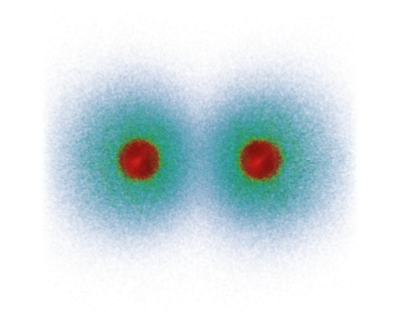
\includegraphics[scale=0.4]{../Graphics/OBD/OBD_MOL/Be2_3D.png}} 
   \subfigure{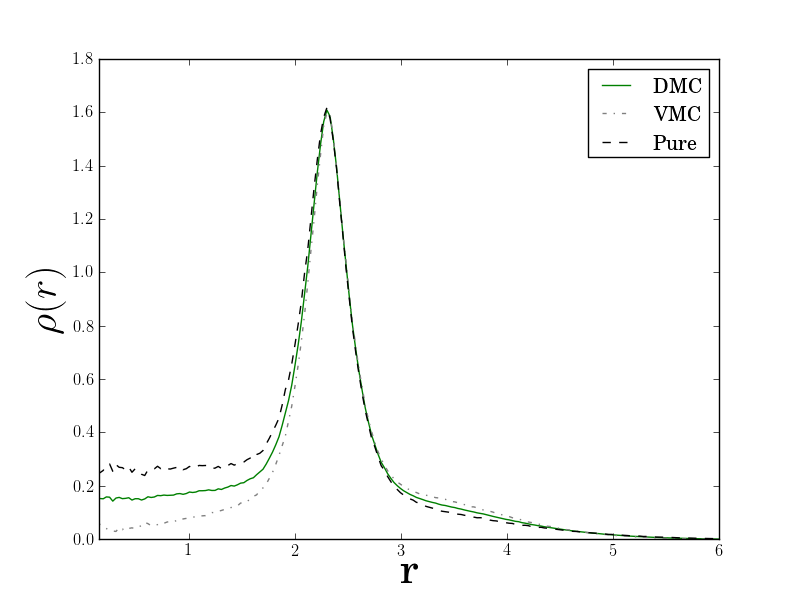
\includegraphics[scale=0.3]{../Graphics/OBD/OBD_MOL/Be2_2D.png}}  \\
   \subfigure{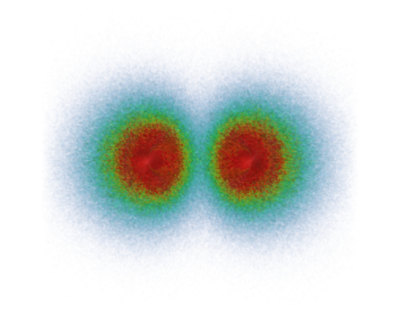
\includegraphics[scale=0.4]{../Graphics/OBD/OBD_MOL/O2_3D.png}} 
   \subfigure{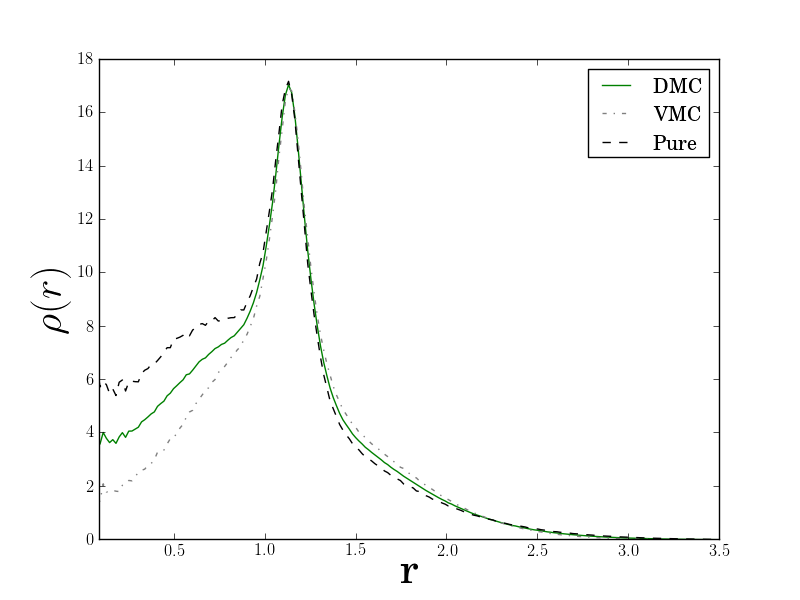
\includegraphics[scale=0.3]{../Graphics/OBD/OBD_MOL/O2_2D.png}}
  \caption{One-body densities of $\mathrm{Li_2}$ (top), $\mathrm{Be_2}$ (middle) and $\mathrm{O_2}$ (bottom). The figures to the left are spherical densities sliced through the middle to reveal the core structure. The figures to the right are radial one-body densities projected on the nucleus-nucleus axis. Red and blue color indicates a high and low electron density respectively. The right-hand figures are symmetric around the origin.}
  \label{fig:OBD_Molecules}
 \end{center}
\end{figure}
\renewcommand\floatpagefraction{.7}

\clearpage
\subsection{Parameterizing Forces}

\begin{figure}
 \begin{center}
  \subfigure{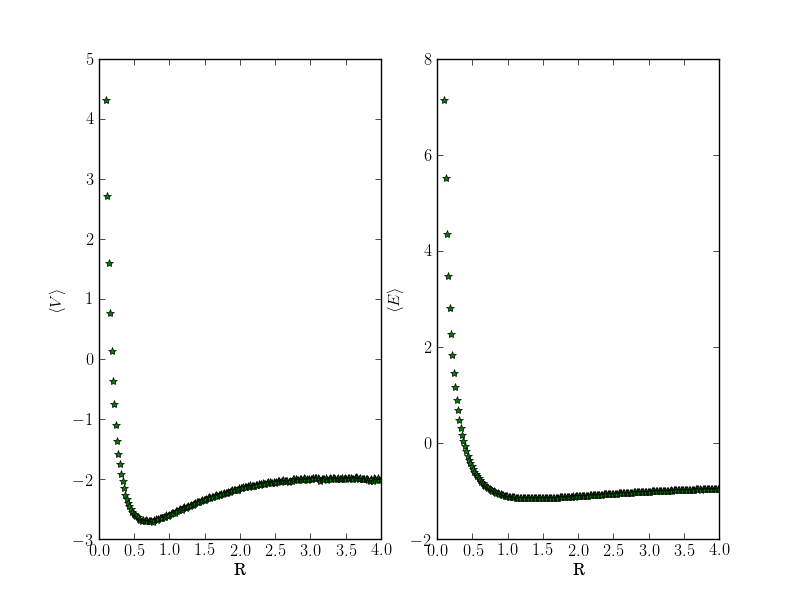
\includegraphics[scale=0.37]{../Graphics/R_VS_E/R_vs_E_hyd_0.png}}
  \subfigure{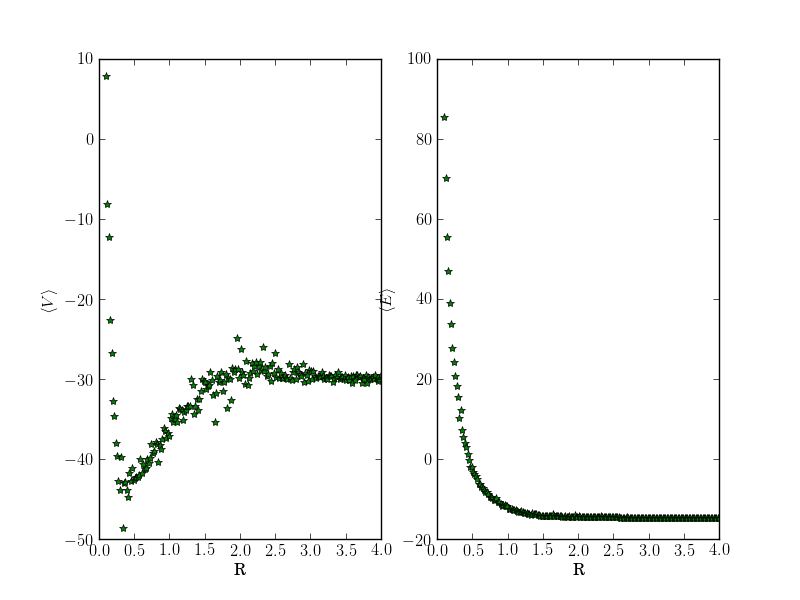
\includegraphics[scale=0.37]{../Graphics/R_VS_E/R_vs_E_lit_0.png}} 
  \caption{The distance between the atoms $R$ vs. the potential and total energy. To the left: $\mathrm{Li_2}$. To the right: $\mathrm{Li_2}$. It is evident that there exist a well-defined minima in the energy in the case of hydrogen gas. For Lithium this is not the case, which corresponds well with the fact that Lithium does not appear naturally in a gas phase in nature, but rather as ionic compounds in other molecules \cite{UniversityPhysics}.}
  \label{fig:molecules_R_vs_E}
 \end{center}
\end{figure}

In molecular dynamics, it is custom to use the Lennard Jones potential as an ansatz to the intermolecular interaction \textbf{referer}. However, using ab-initio equation mechanics, these forces can be parameterized in greater detail, resulting in a more precise molecular dynamics simulation. The quantity of interest is the \textit{force}, that is, the gradient of the potential. However, the potential in molecular dynamics does not correspond to the potential in the Schrödinger equation, due to the fact that the kinetic energy of the electrons is not counted as part of the kinetic energy in the molecular dynamics simulation. Hence the total energy of the Schrödinger equation correspond to the potential in molecular dynamics. In the case of diatomic molecules this is 

\begin{equation}
 \mathbf{F}_\mathrm{MD} = \frac{\mathrm{d}E}{\mathrm{d}R}.
\end{equation}


Using the Hellmann-Feynman theorem, expressions for this derivative can be deduced \textbf{referer}, however, as a simple approximation, the slope of the energy in Figure \ref{fig:molecules_R_vs_E} can be estimated using e.g. a finite difference calculation. Figure \ref{fig:molecules_R_vs_E} and Figure LENNARD are clearly similar, indicating that...

For more complicated molecules, the force can be found as a function of angles, radii, etc. which in turn can be used to parameterize a more complicated molecular dynamics potential. An example of such a potential is the REAXFF potential, which is based on Quantum Mechanical calculations involving five atoms \textbf{referer}.


